\documentclass[../thesis.tex]{subfiles}



\begin{document}
	
% set hydrogen bonding charakteristics %from https://tex.stackexchange.com/questions/577565/how-to-draw-a-dotted-hydrogen-bond-with-chemfig
\makeatletter % from: https://tex.stackexchange.com/a/101263/134144
\tikzset{
	dot diameter/.store in=\dot@diameter,
	dot diameter=1pt,
	dot spacing/.store in=\dot@spacing,
	dot spacing=3.0pt,
	dots/.style={
		line width=\dot@diameter,
		line cap=round,
		dash pattern=on 0pt off \dot@spacing
	}
}
\makeatother

\chapter{Theoretische Grundlagen}
\label{chp: grundlagen}

\section{Thermodynamisches Modell}

Thermodynamische Modelle dienen dazu den Zustand eines Systems mit Hilfe von mathematischen Gleichungen zu beschreiben \cite{atkins2006atkins}. Diese so genannten Zustandsgleichungen stellen einen Zusammenhang zwischen den Zustandsgrößen, welche den Zustand eines Systems eindeutig beschreiben, her. Die Größen sind meistens der Druck $p$, die Temperatur $T$ und das molare Volumen $v$. Falls zwei dieser drei Größen gegeben sind kann die Unbekannte berechnet werden. Zustandsgleichungen haben meistens folgende Form:
\begin{equation}
	p = f(T,v)
\end{equation}

Beispiele für solche Zustandsgleichungen sind die Volume Translated Peng Robinson (\texttt{VTPR}) \cite{ahlers2002development} oder die prädiktive Soave-Redlich-Kwong (\texttt{PSRK}) \cite{HOLDERBAUM1991251} welche in dieser Arbeit verwendet wird.

\section{Zustandsgleichung prädiktive Soave-Redlich-Kwong}

Der Benchmark wird in dieser Arbeit beispielhaft mit dem in \texttt{TREND} bereits vorhanden thermodynamischen Modell \texttt{PSRK} durchgeführt. In diesem Abschnitt werden die Berechnungsgrundlagen für dieses Modell erläutert.

Die \texttt{PSRK} hat folgende Basisform \cite{HOLDERBAUM1991251}:
\begin{equation}
	p = \dfrac{R \cdot T}{v - b}- \dfrac{a(T)}{v \cdot (v + b)}
\end{equation}

Die Variable $ p $ beschreibt in dieser Gleichung den Druck, $ T $ die Temperatur und $ v $ das molare Volumen. $ R $ ist die universale Gaskonstante. Der Parameter $a$ ist der Kohäsionsparameter und $ b $ ist das Kovolumen. Das Kovolumen $ b $ wird über eine lineare Mischungsregel aus den Reinstoffgrößen wie in \autoref{eq: par_b} gezeigt berechnet.

\begin{equation}
	b = \sum \left( x_i \cdot b_i \right)
	\label{eq: par_b}
\end{equation}

Die Reinstoffgrößen $ b_i $ werden nach \autoref{eq: par_bi} aus den kritischen Stoffgrößen für jede Komponente im Gemisch berechnet.

\begin{equation}
	b_i = 0\text{.}08664 \cdot \dfrac{R \cdot T_{\mathrm{c},i}}{p_{\mathrm{c},i}}
	\label{eq: par_bi}
\end{equation}

$ T_{\mathrm{c},i} $ ist die kritische Temperatur und $ p_{\mathrm{c},i} $ der kritische Druck der Komponente $ i$.

Der Kohäsionsparameter $a$ kann mit folgender Gleichung aus \cite{horstmann2005psrk} berechnet werden.

\begin{equation}
	\dfrac{a(T)}{bRT} =	\dfrac{\dfrac{g^{\mathrm{E}}_0}{RT} +  \sum \left( x_i \cdot \mathrm{ln}\dfrac{b}{b_i} \right)}{\mathrm{ln}\dfrac{u}{u + 1}}
	+ \sum \left( x_i \cdot \dfrac{a_i(T)}{b_i \cdot RT} \right) \text{ mit } u = \dfrac{v}{b}
\end{equation}

$ g^{\mathrm{E}}_0 $ beschreibt die Gibbs-Energie und wird mit dem Gruppenbeitragsmodell UNIFAC \cite{magnussen1981unifac} berechnet. Die temperaturabhängige Variable $a_i$ kann mit folgenden Zusammenhängen beschrieben werden.

\begin{equation}
	a_i(T) = 0\text{.}42748 \dfrac{R^2 \cdot T_{\mathrm{c},i}^2}{p_{\mathrm{c},i}} \cdot f(T) \\
\end{equation}

\begin{equation}
	f(T) = \left[1 + c_1 \cdot X + c_2 \cdot X^2 + c_3 \cdot X^3 \right]^2
\end{equation} 

Die Parameter $ c_1 $ bis $ c_3 $ sind stoffspezifisch und können Tabellen aus \cite{horstmann2005psrk} entnommen werden. Die Hilfsvariable $ X$ kann mit dem in \autoref{eq: a_i_sup} gezeigten Zusammenhang aus der reduzierten Temperatur $T_\mathrm{r}$ berechnet werden.

\begin{equation}
	X = \left( 1 - T_\mathrm{r}^{0\text{.}5} \right) \text{ mit } T_\mathrm{r} = \dfrac{T}{T_\mathrm{c}}
	\label{eq: a_i_sup}
\end{equation}

\section{Bewertung thermodynamischer Modelle}

Um thermodynamische Modelle bewerten zu können wird das Modell anhand von experimentell ermittelten Daten getestet und die Bewertung nach dem in \cite{jaubert2020benchmark} beschriebenen Ansatz vorgenommen. In dem beschriebenen Ansatz wird die Bewertung des Modells anhand von Daten aus Experimenten, welche für einen großen Temperatur- und Druckbereich für verschiedenste binäre Stoffgemische vorliegen durchgeführt. Um eine möglichst objektive Bewertung möglich zu machen, wurden die Stoffe und Gemische nach dem in \cite{jaubert2020benchmark} beschriebenen Ansatz, zunächst klassifiziert und dann für alle Klassen experimentelle Daten ausgewählt. Hierbei ist zu beachten, dass alle Klassen gleichmäßig in den Daten vertreten sind um eine gleichmäßig gewichtete Bewertung vornehmen zu können.
Die Bewertung des thermodynamischen Modells geschieht anhand der Abweichung der experimentellen von den errechneten Daten des Modells.
In den folgenden Abschnitten werden das Vorgehen zur Datenauswahl und die Bewertung eines Modells näher erläutert.

\subsection{Stoffklassifikation nach Jaubert et al.}
\label{sec: klassifikation}

Die vorgenommene Stoffklassifikation unterteilt die Stoffe anhand ihres Assoziationscharakters. Diese Eigenschaft beschreibt die Fähigkeit der Wasserstoffbrückenbildung. Es wurden vier verschiedene Kategorien erstellt, welche nun genauer beschrieben werden.

\subsubsection{Nicht assoziierende Stoffe}

Nicht assoziierende Stoffe besitzen keine Fähigkeit Wasserstoffbrückenbindungen zu bilden. Diese Stoffe besitzen, wie in \autoref{fig: NA-bsp} dargestellt, keine freies Elektronenpaar, welches für eine Wasserstoffbrückenbindung benötigt wird.

\begin{figure}[htbp]
	\centering
	\setchemfig{atom sep=9mm}
	\schemestart
		\chemfig{H-[:0]C(-[:90]H)(-[:0]H)(-[:-90]H)}
		\arrow{0}[0,1]
		\chemfig{H-[:0]C(-[:90]H)(-[:-90]H)(-[:0]C(-[:0]H)(-[:90]H)(-[:-90]H))}
	\schemestop
	\caption{Methan (links) und Ethan (rechts) als Beispiele nicht assoziierender Stoffe}
	\label{fig: NA-bsp}
\end{figure}

\subsubsection{Wasserstoff akzeptierende Stoffe}

Wasserstoff akzeptierende Stoffe weisen im Gegensatz zu den nicht assoziierenden Stoffen eine freies Elektronenpaar auf. Mit diesem freien Elektronenpaar kann das Molekül mit einem Wasserstoffatom eines anderen Moleküls eine Wasserstoffbrückenbindung eingehen. Als Beispiel für einen solchen Stoff ist  $\mathrm{CO_2}$ in \autoref{fig: HA-bsp} dargestellt.

\begin{figure}[htbp]
	\centering
	\setchemfig{atom sep=9mm}
	\schemestart
	\chemfig{
		\charge{135=\|,-135=\|}{O}=C=\charge{45=\|,-45=\|}{O}-[:0,,,,,dots,red]H-[:45]\charge{45=\|,135=\|}{O}-[:-45]H}
	\schemestop
	\caption{$\mathrm{CO_2}$ (links)  als Beispiel für einen Wasserstoff akzeptierenden Stoff}
	\label{fig: HA-bsp}
\end{figure}

\subsubsection{Wasserstoff bereitstellende Stoffe}

Wasserstoff bereitstellende Stoffe haben mindestens ein partiell positiv geladenes Wasserstoffatom mit dem eine Wasserstoffbrückenbindung eingegangen werden kann. Das Molekül Trifluormethan in \autoref{fig: HD-bsp} ist ein Beispiel dieser Stoffklasse.

\begin{figure}[htbp]
	\centering
	\setchemfig{atom sep=9mm}
	\schemestart
	\chemfig{C(-[:-180]F)(-[:90]F)(-[:-90]F)(-H-[:0,,,,,dots,red]{\charge{135=\|,-135=\|}{O}}(-[:45]H)(-[:-45]H))}
	\schemestop
	\caption{Trifluormethan (links) als Beispiel für einen Wasserstoff bereitstellenden Stoff}
	\label{fig: HD-bsp}
\end{figure}

\subsubsection{Selbstassoziierende Stoffe}

Stoffe die mit sich selbst eine Wasserstoffbrückenbindung eingehen können werden selbstassoziierend genannt. Sie weisen sowohl ein freies Elektronenpaar als auch ein partiell positiv geladenes Wasserstoffatom auf. Als Beispiel ist das Molekül Wasser in \autoref{fig: SA-bsp} dargestellt.

\begin{figure}[htbp]
	\centering
	\setchemfig{atom sep=9mm}
	\schemestart
	\chemfig{H-[:45]{\charge{45=\|,135=\|}{O}}-[:-45]H-[:0,,,,,dots,red]{\charge{135=\|,-135=\|}{O}}(-[:45]H)(-[:-45]H)}
	\schemestop
	\caption{Wasser als Beispiel für einen selbstassoziierenden Stoff}
	\label{fig: SA-bsp}
\end{figure}

\subsubsection{Gemischklassifikation}
\label{sec: gemischklassifikation}

Mit der Klassifikation der Stoffe nach ihrer Assoziativität gegenüber Wasserstoff, können Gemische aus 2 Stoffen in 9 verschiedene Gruppen unterteilt werden. Eine Darstellung der Zuordnungen für binäre Gemische ist in \autoref{tab: bin-bac} zu sehen.

\begin{table} [htb]
	\centering
	\caption{binäre Gemischkombinationen von Assoziativitäten}
	\begin{tabular}{ ccccc }
		\hline 
		BAC & Stoff 1 & Stoffe 2 & Klasse & Abkürzung\\
		\hline % \\ [\dimexpr-\normalbaselineskip+2pt]
		1  & nicht assoziierend & nicht assoziierend & 1 & NA\\
		2  & nicht assoziierend & Wasserstoff akzeptierend & 1 & NA \\
		3  & nicht assoziierend & Wasserstoff bereitstellend & 1 & NA \\
		4  & Wasserstoff bereitstellend & Wasserstoff bereitstellend & 1 & NA \\
		4  & Wasserstoff akzeptierend & Wasserstoff akzeptierend & 1 & NA \\
		5  & nicht assoziierend & selbst assoziierend & 2 & SA\\
		6  & Wasserstoff bereitstellend & Wasserstoff akzeptierend & 3 & CA \\
		7  & Wasserstoff bereitstellend & selbst assoziierend & 4 & CA+SA \\
		8  & Wasserstoff akzeptierend & selbst assoziierend & 4 & CA+SA\\
		9  & selbst assoziierend & selbst assoziierend & 4 & CA+SA \\
%		[\dimexpr-\normalbaselineskip+23pt]
		\hline
		\label{tab: bin-bac}
	\end{tabular}
\end{table}

Der \textbf{B}inary \textbf{A}ssociation \textbf{C}ode (BAC) dient der Unterscheidung der verschiedenen Kombinationen. Diese Kombinationen können weiter zusammengefasst werden, sodass 4 Klassen entstehen.

In der ersten Klasse befinden sich Gemische die keine Assoziation aufweisen. Sie haben entweder mindestens einen nicht assoziierenden Stoff oder bestehen nur aus Stoffen mit Wasserstoff bereitstellendem oder akzeptierendem Charakter. In dieser Klasse treten kaum Wechselwirkungen zwischen den Molekülen auf.

In der zweiten Klasse befinden sich Gemische, welche aus einem nicht assoziierenden Stoff und einem selbst assoziierenden Stoff bestehen. In diesen Gemischen tritt Selbstassoziation auf. Der nicht assoziierende Stoff stört die Wasserstoffbrückenbindungen und löst bestehende Bindungen teilweise wieder auf. Als Resultat dieses Phänomens entstehen oft partielle Mischungslücken \cite{jaubert2020benchmark}. Gemische aus Wasser und Alkanen oder Alkohol und Alkanen sind Beispiele für Gemische dieser Klasse.

In der dritten Klasse befinden sich Gemische, die eine Wasserstoffbrückenbildung zwischen den beteiligten Komponenten ermöglichen. Dieses auch ''cross association'' genannte Phänomen tritt ein, wenn ein Stoff mit einem partiell positiv geladenen Wasserstoff Atom mit einem anderen Stoff, welcher ein freies Elektronenpaar hat gemischt wird. Da nur im Gemisch beider Stoffe Wasserstoffbrückenbindungen ausgebildet werden können, unterscheidet sich das Verhalten des Gemischs von dem der Reinstoffe.

In der vierten Klasse befinden sich Gemische, in denen sowohl selbst Assoziation als auch ''cross assoziation'' auftreten können. Das Verhalten dieser Stoffe ist schwer vorherzusagen, da sowohl eine Verstärkung als auch eine Abschwächung des Wasserstoffbrückennetzwerks erfolgen kann \cite{jaubert2020benchmark}.

\subsection{Stoffauswahl}

Bei der Auswahl der Stoffe dient die Bewertung der Abweichung vom idealen Verhalten als Kriterium. Es ist sowohl eine quantitative als auch eine qualitative Bewertung von der Forschergruppe vorgenommen worden.

Für die qualitative Bewertung der Abweichung vom idealen Verhalten wurden folgende Kriterien verwendet:
\begin{itemize}
	\item Molekülgröße
	\item Molekülform
	\item energetische Interaktion (unabhängig von Temperatur, Druck und Zusammensetzung)
\end{itemize}
Ein Gemisch gilt dem gewählt Ansatz nach als qualitativ ideal, wenn die Molekülgröße, -form und energetische Interaktion, für beide der beteiligten Stoffe, ähnliche Werte unabhängig von Temperatur, Druck oder Zusammensetzung aufweisen.
Um eine möglichst gleichmäßige Verteilung zwischen sich ideal verhaltenden und vom Idealverhalten abweichende Stoffe in den Daten zu gewährleisten, beinhaltet jede BAC Gruppe etwa 20 binäre Systeme.
Die Abweichung kann durch alle drei genannten Kriterien hervorgerufen werden. Ist die Abweichung vom Idealverhalten nur durch eine Differenz in der Molekülgröße hervorgerufen, ist die Exzess-Enthalpie $h^{\mathrm{E}}$ vernachlässigbar und das Gemisch wird als \textit{athermisch} bezeichnet. Aus der Tatsache, dass die Exzess-Enthalpie vernachlässigbar ist resultiert, dass die Gibbs-Energie $g^{\mathrm{E}}$ proportional zur Exzess-Entropie des Gemisches ist.

\begin{equation}
	g^E \approx - T \cdot s^{\mathrm{E}}
\end{equation}   
Die Abweichung ist somit durch entropische Effekte zu erklären.

Ist die Abweichung nur durch eine Differenz in der energetischen Interaktion der beteiligten Komponenten hervorgerufen, ist die Exzess-Entropie $s^{\mathrm{E}}$ vernachlässigbar und das Gemisch wird als \textit{regulär} klassifiziert. Durch die Vernachlässigung der Exzess-Entropie entsteht ein proportionaler Zusammenhang zwischen der Gibbs-Exzess Energie und der Exzess-Enthalpie.
\begin{equation}
	g^{\mathrm{E}} \approx h^{\mathrm{E}}
\end{equation}
In diesem Fall sind enthalpische Effekte der Ursprung der Abweichung.

Sowohl entropische, als auch enthalpische Effekte können in nichtidealen Gemischen der Ursprung für auftretende Abweichungen sein. Die Datenbank enthält sowohl Gemische mit rein entropisch bedingter, als auch Gemische mit rein enthalpisch bedingter, sowie Gemische mit entropisch und enthalpisch bedingter Abweichung.

Für die Bestimmung der quantitativen Abweichung vom idealen Verhalten werden folgende Berechnungsgrößen verwendet:
\begin{itemize}
	\item Gibbs-Energie $g^{\mathrm{E}}$
	\item Enthalpie $h^{\mathrm{E}}$
	\item Entropie $s^{\mathrm{E}}$
\end{itemize}

Um die benötigten Größen berechnen zu können werden die Aktivitätskoeffizienten aus experimentell erhobenen Dampf-Flüssigkeits-Gleichgewichts Daten berechnet. Dazu wird der $\gamma$-$\varphi$ Ansatz verwendet. Um diesen Ansatz herzuleiten wird das Raoult-sche Gesetz als Basis verwendet.
\begin{equation}
	\label{eq: raoult_base}
	y_i \cdot P = P_{i}^{\mathrm{sat}} \cdot x_i
\end{equation}

In dem hier gewählten Ansatz wird die Dampfphase als ideal angenommen, sodass die linke Seite von \autoref{eq: raoult_base} bestehen bleibt. Die Flüssigphase wird als nicht-ideal angenommen und es wird der Korrekturfaktor $\gamma_i$ eingeführt. Dieser Korrekturfaktor $\gamma_i$ wird auch Aktivitätskoeffizient genannt. 
\begin{equation}
	\label{eq: raoult_mod}
	y_i \cdot P = P_{i}^{\mathrm{sat}} \cdot x_i \cdot \gamma_i
\end{equation}

Der Faktor $\gamma_i$ beschreibt die Abweichung vom Idealverhalten in der Flüssigphase. Im Falle eines sich in der Flüssigkeit ideal verhaltenden Stoffgemisches gilt $\gamma_i = 1$. \autoref{eq: raoult_mod} kann nach dem Aktivitätskoeffizienten umgeformt werden. Für einen experimentell erhobenen Datenpunkt gilt dann:
\begin{equation}
	\gamma_i \left(T,x \right) = \dfrac{P_{\mathrm{exp}} \cdot y_{i,\mathrm{exp}}}{P_{i}^{\mathrm{sat}}(T_{\mathrm{exp}}) \cdot x_{i,\mathrm{exp}}}
\end{equation}
Die notwendigen temperaturabhängigen Dampfdrücke $P_{i}^{\mathrm{sat}}(T)$ sind der Datenbank des Design Institute for Physical Properties (DIPPR) \cite{thomson1996dippr} entnommen worden.
Um die Gibbs-Energie $g^{\mathrm{E}}$ berechnen zu können wird ein Ansatz des Margules Gibbs-Exzess-Energie Models verwendet. Der Ansatz fittet 4 Parameter anhand von isobaren Dampf-Flüssigkeit Phasengleichgewichtsdaten und ermöglicht so eine temperaturabhängige Berechnung der Gibbs-Energie. Der nötige Ansatz zum Fitten kann aus \autoref{eq: fit_par} hergeleitet werden. Es gilt:
\begin{equation}
	\label{eq: fit_par}
	\mathrm{ln}(\gamma_1) =  \dfrac{\partial }{\partial n_1} \left( \dfrac{g^{\mathrm{E}}(T,x)}{RT} \cdot n \right)
\end{equation}

Die Gibbs-Energie $ g^{\mathrm{E}} $ kann durch folgenden Zusammenhang beschrieben werden:
\begin{equation}
	\dfrac{g^{\mathrm{E}}(T,x)}{RT} = x_1 \cdot x_2 \cdot A(T) 
\end{equation}

\begin{equation}
	A(T) = p_1 - p_2 \cdot T-p_3 \cdot \ln(T)+p_4 \cdot \exp{ \left( \dfrac{1}{T} \right)}
\end{equation}

Die Parameter $ p_1 $ bis $ p_4 $ werden mittels des Fits berechnet.
Die Molenbrüche $ x_1 $ und $ x_2 $ sowie der Gesamtstoffmenge $ n $ können wie folgt ersetzt werden:

\begin{equation}
	x_1 = \dfrac{n_1}{n_1 + n_2}
\end{equation}  
\begin{equation}
	x_2 = \dfrac{n_2}{n_1 + n_2}
\end{equation}  
\begin{equation}
	n = n_1 + n_2
\end{equation}

Die Größen $ n_1 $ und $ n_2 $ beschreiben die Stoffmenge der ersten bzw. zweiten Komponente.

\begin{equation}
	\dfrac{\partial }{\partial n_1} \left( \dfrac{g^{\mathrm{E}}(T,x)}{RT} \cdot n \right) = \dfrac{\partial }{\partial n_1} \left[ 
	\dfrac{n_1}{n} \cdot \dfrac{n_2}{n} \cdot A(T) \cdot n
	 \right]  
\end{equation}

\begin{equation}
	\dfrac{\partial }{\partial n_1} \left[ 
	\dfrac{n_1}{n} \cdot \dfrac{n_2}{n} \cdot A(T) \cdot n
	\right]  = \dfrac{\partial }{\partial n_1} \left[ 
	\dfrac{n_1}{n_1 + n_2} \cdot n_2 \cdot A(T)
	\right] 
\end{equation}

Das Anwenden der Quotientenregel führt zu folgendem Zusammenhang:

\begin{equation}
	\dfrac{\partial }{\partial n_1} \left[ 
	\dfrac{n_1}{n_1 + n_2} \cdot n_2 \cdot A(T) \right] = \dfrac{n_1 + n_2 - n_1}{(n_1 + n_2)^2} \cdot n_2 \cdot A(T) = A(T) \cdot \dfrac{n_2^2}{(n_1 + n_2)^2}
\end{equation}

Es ergibt sich der finale Zusammenhang:
\begin{equation}
	\mathrm{ln}(\gamma_1) = A(T) \cdot x_2^2
\end{equation}

Die Herleitung kann analog für die 2 Komponente durchgeführt werden.
\begin{equation}
	\mathrm{ln}(\gamma_2) = A(T) \cdot x_1^2
\end{equation}

Für das fitten wurde in \cite{jaubert2020benchmark} die gemittelte durchschnittliche Abweichung minimiert. Sobald ein Ansatz für die Gibbs-Exzess-Energie vorliegt lässt sich damit mit \autoref{eq: he_ge} die Enthalpie $h^{\mathrm{E}}$ und \autoref{eq: se} die Entropie $s^{\mathrm{E}}$ berechnen.

\begin{equation}
	\label{eq: he_ge}
	h^{\mathrm{E}} = g^{\mathrm{E}} - T \cdot \left( \dfrac{\partial g^{\mathrm{E}}}{\partial T} \right)_x
\end{equation}

\begin{equation}
	\label{eq: se_ansatz}
	g^{\mathrm{E}} = h^{\mathrm{E}} - T \cdot s^{\mathrm{E}}
\end{equation}
\begin{equation}
	\label{eq: se}
	s^{\mathrm{E}} = - \left( \dfrac{\partial g^{\mathrm{E}}}{\partial T} \right)_x
\end{equation}

Mit Hilfe der berechneten Größen kann ein Gemisch klassifiziert und falls es sich nicht ideal verhält der Ursprung der Abweichung bestimmt werden. Dazu werden die Berechnungsgrößen bei einer Zusammensetzung von $x=\text{0.5}$ berechnet und anhand der resultierenden Werte die Einteilung vorgenommen. Wie die Einteilung genau erfolgt ist in \autoref{fig: klassifikation} dargestellt.

\begin{figure}[htbp]
	\centering
	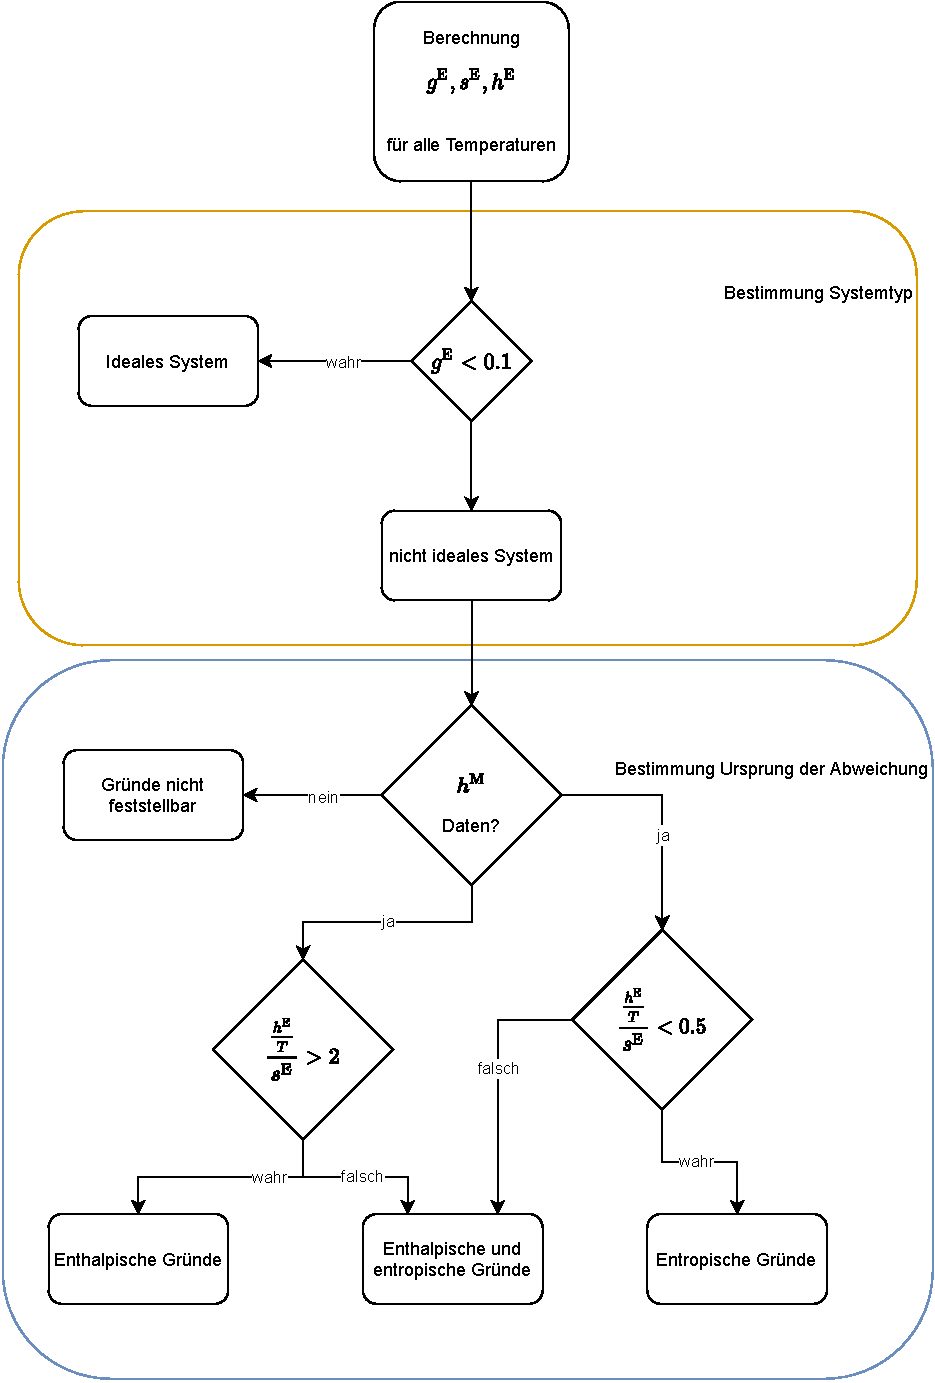
\includegraphics[scale=0.9]{Idealverhalten.pdf}
	\caption{Routine zur Bestimmung des Verhalten eines Gemischs und des Ursprungs der Abweichung}
	\label{fig: klassifikation}
\end{figure}

Dieses Vorgehen zur Bewertung des Verhaltens kann zusätzlich zur Gemischauswahl, welche bereits durchgeführt wurde, zur Weiterentwicklung des bewerteten Modells dienen. Der Ursprung der Abweichung, falls dieser berechnet werden kann, zeigt an welcher Stelle noch Verbesserung notwendig sind.  

\subsection{Bewertungskriterien und Bewertungsgrößen}

Um zwei Zustandsgleichungen miteinander zu vergleichen werden beide mit experimentellen Daten verglichen und die Abweichung von diesen als Bewertungskriterium benutzt. Der Vergleich mit experimentellen Daten wird im folgenden Abschnitt erläutert.

Zum Vergleich eines thermodynamischen Modells mit experimentellen Daten werden folgende Größen verwendet:
\begin{itemize}
	\item kritischer Druck $ p_\mathrm{c} $
	\item kritische Zusammensetzung $ x_\mathrm{c} $
	\item azeotroper Druck $ p_\mathrm{az} $
	\item azeotrope Zusammensetzung $ x_\mathrm{az} $
	\item Zusammensetzung Flüssigphase $ x $
	\item Zusammensetzung Dampfphase (oder zweite Flüssigphase) $ y $
	\item 3-Phasen-Druck $p_{\mathrm{LLV}}$
	\item 3-Phasen-Zusammensetzung $z_{\mathrm{LLV}}$
	\item Mischungsenthalpie $h^{\mathrm{M}}$
	\item Mischungswärmekapazität $c_p^{\mathrm{M}}$
\end{itemize}

Aufgrund der Gibbs'schen Phasenregel ergibt sich für alle Größen ein Freiheitsgrad > 0 sodass hierfür mindestens eine Größe festgelegt werden muss um die unbekannten berechnen zu können. Beispielhaft ist die Berechnung der Freiheitsgrade für das Phasengleichgewicht eines binären Gemischs in \autoref{eq: gibb x_phase} beschrieben. Im Falls des Phasengleichgewichts liegen für ein binäres Gemisch 2 Komponenten und 2 Phasen (Flüssig- und Dampfphase) vor.

\begin{equation}
	\label{eq: gibb x_phase}
	f = K - P + 2 = 2 - 2 + 2 = 2
\end{equation}

$ K $ beschreibt die Anzahl der Komponenten und $ P $ die Anzahl der Phasen im Gemisch.

In \autoref{tab: DoF} sind die festgelegten und berechneten Größen analog zu Tabelle 13 aus \cite{jaubert2020benchmark} aufgeführt.

\begin{table} [htb]
	\centering
	\caption{Festgelegten und berechneten Größen für ein binäres System}
	\begin{tabular}{ cccc }
		\hline 
		Größe & Freiheitsgrad & festgelegte Größen & berechnete Größen\\
		\hline  \\ 
		[\dimexpr-\normalbaselineskip+2pt]
		kritischer Druck  & 1 &$T_{\mathrm{c}}$ & $p_{\mathrm{c}},x_{\mathrm{c}}$  \\
		kritische Zusammensetzung  & 1 &$T_{\mathrm{c}}$ & $p_{\mathrm{c}},x_{\mathrm{c}}$  \\
		azeotroper Druck  & 1 &$T$ & $p,x_1$  \\
		azeotrope Zusammensetzung  & 1 &$T$ & $p,x_1$  \\
		Zusammensetzung Flüssigphase & 2 & $T,p$ & $x_1,y_1$ \\
		Zusammensetzung Dampfphase & 2 & $T,p$ & $x_1,y_1$ \\
		3-Phasen-Druck & 1 & $ T $ &  $p_{\mathrm{LLV}}$ \\
		3-Phasen-Zusammensetzung & 1 & $T$ & $x_1^{\alpha},x_1^{\beta},y_1$ \\
		Mischungsenthalpie & - & $T,p,z_1$ & $h^{\mathrm{M}}$ \\
		Mischungswärmekapazität & - & $T,p,z_1$ & $c_{p}^{\mathrm{M}}$ \\
		[\dimexpr-\normalbaselineskip+18pt]
		\hline
		\label{tab: DoF}
	\end{tabular}
\end{table}

$ x_i$ , $ y_i$, $ z_i$ beschreiben Zusammensetzungen, wobei $x_i^{\alpha} $ und $ x_i^{\beta} $ die Zusammensetzungen der ersten und zweiten Flüssigphase im Falles eines 3-Phasengleichgewichts bezeichnen.  

Diese Größen werden für jedes Stoffgemisch falls möglich berechnet und mit den experimentellen Daten, falls sie erhoben worden sind, verglichen. Aus den Abweichung der Werte werden für jeden BAC Gruppe Noten berechnet und schließlich die Gesamtnote aus den Teilnoten ermittelt. Wie die genaue Berechnung funktioniert ist in \autoref{chp: notenberechnung} beschrieben. 

\section{Notenberechnung}
\label{chp: notenberechnung}

In diesem Kapitel wird auf die Berechnung der Gesamtnote eines thermodynamischen Modells und auf die Berechnung der einzelnen, dafür notwendigen, Teilnoten eingegangen.

\subsection{Berechnung der Gesamtnote}
Die maximale Punktzahl die ein Modell ereichen kann ist auf 20 festgelegt. Die Gesamtnote wird aus vier einzelnen Teilnoten berechnet. Diese vier Teilnoten werden für jede Klasse aus \autoref{tab: bin-bac} berechnet.

\begin{equation}
	\mathrm{mark}_{\mathrm{final}} = \dfrac{1}{4} \cdot \left( 
		\mathrm{mark}_{\mathrm{NA}} + \mathrm{mark}_{\mathrm{SA}} + \mathrm{mark}_{\mathrm{CA}} + \mathrm{mark}_{\mathrm{CA + SA}} 
	 \right)
	 \label{eq: mark_final}
\end{equation}

Die einzelnen Teilnoten wie z.B. $\mathrm{mark}_{\mathrm{NA}}$ entsprechen den Noten der in \autoref{tab: bin-bac} aufgeführten Klassen. Die Noten der einzelnen Klassen berechnen sich aus den Mittelwerten der Noten der BAC Gruppen. Die Note für nicht-assoziierende Gemische lässt sich beispielsweise wie folgt berechnen:

\begin{equation}
	\mathrm{mark}_{\mathrm{NA}} = \dfrac{1}{4} \cdot \left(
		\mathrm{mark}_{\mathrm{BAC_1}} + \mathrm{mark}_{\mathrm{BAC_2}} + \mathrm{mark}_{\mathrm{BAC_3}} + \mathrm{mark}_{\mathrm{BAC_4}}
	\right)
\end{equation}

Die Berechnung der Noten der drei weiteren Klassen erfolgt analog mit der in \autoref{tab: bin-bac} dargestellten Einteilung.

\subsection{Berechnung des gemittelten durchschnittlichen Fehlers}
In diesem Abschnitt wird die Berechnung des gemittelten durchschnittlichen Fehlers gezeigt, welcher auch als \textbf{M}ean \textbf{A}verage \textbf{P}ercantage \textbf{E}rror oder kurz MAPE bezeichnet wird. Der MAPE kann mit folgender Formel berechnet werden:

\begin{equation}
	\mathrm{MAPE}_X(\%) = 100 \cdot \dfrac{1}{n} \cdot \sum_{i=1}^{n} \biggl| \dfrac{X_i^\mathrm{EXP} - X_i^\mathrm{MODEL}}{X_i^\mathrm{MODEL}} \biggr|
	\label{MAPE Glg}
\end{equation}

Die Variable $n$ beschreibt die Anzahl der Messpunkte. $X_i^\mathrm{MODEL}$ steht für den vom Modell berechneten Wert und $X_i^\mathrm{EXP}$ für den zugehörigen experimentellen Messwert.

\subsection{Berechnung der Noten für die Bewertungsgrößen}
Die einzelnen Teilnoten werden aus den Noten der jeweiligen Bewertungsgrößen bestimmt.
\\

Die Note für den kritischen Druck errechnet sich mit folgendem Zusammenhang.
\begin{equation}
	\mathrm{mark}_{p_{\mathrm{c}}} = 20 - 0,75 \cdot \mathrm{MAPE}_{p_\mathrm{c}}(\%)
\end{equation}
Damit die berechneten Ergebnisse nicht negativ werden, wird der MAPE bei folgender Bedingung abgeschnitten:

\begin{equation}
	\mathrm{MAPE}_{p_\mathrm{c}}(\%) = \dfrac{80}{3} \text{ wenn } \mathrm{MAPE}_{p_\mathrm{c}}(\%) > \dfrac{80}{3}
\end{equation}

$ p_\mathrm{c} $ ist der Druck am kritischen Punkt. Die Limitierung des MAPEs ist dem in \cite{jaubert2020benchmark} beschrieben Ansatz hinzugefügt worden um Noten außerhalb des Gültigkeitsbereich auszuschließen.
\\

Die Note für die kritische Zusammensetzung wird nach \autoref{eq: mark_x_c} berechnet.
\begin{equation}
\label{eq: mark_x_c}
\mathrm{mark}_{x_\mathrm{c},y_\mathrm{c}} = 20 - 0,5 \cdot \left[
	\dfrac{\mathrm{MAPE}_{x_{1,\mathrm{c}}}(\%) + \mathrm{MAPE}_{x_{2,\mathrm{c}}}(\%)}{2}
\right]
\end{equation}

Die Größen $ x_{1,\mathrm{c}} $ und $ x_{2,\mathrm{c}} $ beschreiben die Molenbrüche in der Flüssigkeit am kritischen Punkt. Die Zusammensetzung der Gasphase ist in diesem Punkt identisch mit der der Flüssigphase und muss deshalb nicht gesondert betrachtet werden.
\\

Für den azeotropen Druck kann die Note wie folgt berechnet werden.
\begin{equation}
	\mathrm{mark}_{p_{\mathrm{az}}} = 20 - 0,5 \cdot \mathrm{MAPE}_{p_\mathrm{az}}(\%)
\end{equation}
Um auch hier keine Noten kleiner 0 zuzulassen wird der MAPE auch hier limitiert.

\begin{equation}
	\label{eq: pheq_x_lim}
	\mathrm{MAPE}_{p_\mathrm{az}}(\%) = 40 \text{ wenn } \mathrm{MAPE}_{p_\mathrm{az}}(\%) > 40
\end{equation}

$ p_\mathrm{az} $ bezeichnet den Druck am azeotropen Punkt.
\\

Für die azeotrope Zusammensetzung gilt folgender Zusammenhang.
\begin{equation}
\mathrm{mark}_{x_\mathrm{az},y_\mathrm{az}} = 20 - 0,5 \cdot \left[
	\dfrac{\mathrm{MAPE}_{x_{1,\mathrm{az}},y_{1,\mathrm{az}}}(\%) + \mathrm{MAPE}_{x_{2,\mathrm{az}},y_{2,\mathrm{az}}}(\%)}{2}
\right]
\end{equation}
Für den $ \mathrm{MAPE}_{x_{1,\mathrm{az}},y_{1,\mathrm{az}}}(\%) $ sowie $ \mathrm{MAPE}_{x_{2,\mathrm{az}},y_{2,\mathrm{az}}}(\%) $ gelten die gleichen Rahmenbedingungen wie in \autoref{eq: pheq_x_lim} beschrieben. Auch diese sind dem Ansatz nach \cite{jaubert2020benchmark} hinzugefügt worden. Die Größen $ x_{1,\mathrm{az}} $ und $ y_{1,\mathrm{az}} $ beschreiben die Molenbrüche der ersten Komponente in der Flüssig- und der Gasphase am azeotropen Punkt. 
\\

Die Noten für die Phasengleichgewichtsgrößen werden mit folgender Gleichung bestimmt.
\begin{equation}
	\mathrm{mark}_{x,y} = 20 - 0,5 \cdot \left[
		\dfrac{\mathrm{MAPE}_{x_1,y_1}(\%) + \mathrm{MAPE}_{x_2,y_2}(\%)}{2}
	\right]
\end{equation}

Auch hier gelten die zusätzlich hinzugefügten Limitierungen aus \autoref{eq: pheq_x_lim}.
$x_1$ ist die Zusammensetzung der ersten und $x_2$ die des zweiten Stoffs in der Flüssigphase. Die Größen $ y $ beschreiben die Zusammensetzung in der Gasphase.
\\

Die Note für die Mischungsenthalpie $ h^{\mathrm{M}} $ wird aus den Abweichungen der einzelnen Datenpunkte nach \autoref{eq: mark_hm} errechnet.
\begin{equation}
\mathrm{mark}_{h^{\mathrm{M}}} = 20 - 0,25 \cdot \dfrac{1}{n_{h^{\mathrm{M}}}} \sum_{i=1}^{n_{h^{\mathrm{M}}}}
	\dfrac{1}{2} \cdot \left[
		100 \cdot \biggl|
			\dfrac{h_i^{\mathrm{M,EXP}}-h_i^{\mathrm{M,MODEL}}}{h_i^{\mathrm{M,EXP}}} 
			\biggl| 
			+ 100 \cdot \biggl| \dfrac{h_i^{\mathrm{M,EXP}}-h_i^{\mathrm{M,MODEL}}}{h_i^{\mathrm{M,MODEL}}}
		\biggl|
	\right]
\label{eq: mark_hm}
\end{equation}

Um Noten die kleiner als null werden auszuschließen wird für Abweichungen aus dem Term
\begin{equation}
	\label{eq: h_m MAPEs}
	\dfrac{1}{2} \cdot \left[
	100 \cdot \biggl|
	\dfrac{h_i^{\mathrm{M,EXP}}-h_i^{\mathrm{M,MODEL}}}{h_i^{\mathrm{M,EXP}}} 
	\biggl| 
	+ 100 \cdot \biggl| \dfrac{h_i^{\mathrm{M,EXP}}-h_i^{\mathrm{M,MODEL}}}{h_i^{\mathrm{M,MODEL}}}
	\biggl| \right] > 80
\end{equation}
die Abweichung auf 80 \% festgesetzt. Dies führt zu einer Note von 0/20 für Punkte, welche die Bedingung erfüllen. Eine weitere zu beachtende Einschränkung ist, dass große Abweichungen des Modellwerts vom experimentell ermittelten Wert, abhängig davon ob sie nach oben oder unten abweichen, zu unterschiedlichen prozentualen Abweichungen führen.
Als Beispiel sind zwei verschieden Fälle zu betrachten
\begin{enumerate}
	\item $ h_i^{\mathrm{M,EXP}} = 10 \mathrm{\frac{J}{mol}} $ und $ h_i^{\mathrm{M,MODEL}} = 1000 \mathrm{\frac{J}{mol}} $
	\item $ h_i^{\mathrm{M,EXP}} = 1000 \mathrm{\frac{J}{mol}} $ und $ h_i^{\mathrm{M,MODEL}} = 10 \mathrm{\frac{J}{mol}} $
\end{enumerate}
Die Ergebnisse der Berechnung des MAPE sind nach dem in \autoref{MAPE Glg} gezeigten Ansatz wie folgt:
\begin{eqnarray}
\mathrm{MAPE}_1 = 99\% \\
\mathrm{MAPE}_2 = 9900 \%
\end{eqnarray}

Um dieses Problem zu beheben wird der Mittelwert aus zwei MAPE wie in \autoref{eq: h_m MAPEs} gezeigt berechnet.
\\

Die Note für die spezifische isobare Wärmekapazität wird mit dem gleichen Vorgehen, wie bei der Mischungsenthalpie berechnet.
\begin{equation}
\mathrm{mark}_{c_p{\mathrm{M}}} = 20 - 0,10 \cdot \dfrac{1}{n_{c_p{\mathrm{M}}}} \sum_{i=1}^{n_{c_p{\mathrm{M}}}}
\dfrac{1}{2} \cdot \left[
100 \cdot \biggl|
\dfrac{c_{p,i}^{\mathrm{M,EXP}}-c_{p,i}^{\mathrm{M,MODEL}}}{c_{p,i}^{\mathrm{M,EXP}}} 
\biggl| 
+ 100 \cdot \biggl| \dfrac{c_{p,i}^{\mathrm{M,EXP}}-c_{p,i}^{\mathrm{M,MODEL}}}{c_{p,i}^{\mathrm{M,MODEL}}}
\biggl|
\right]
\label{eq: cp MAPEs}
\end{equation}
Um auch hier keine Noten kleiner als null zuzulassen, wird für alle Punkte, welche die Bedingung 
\begin{equation}
\dfrac{1}{2} \cdot \left[
100 \cdot \biggl|
\dfrac{c_{p,i}^{\mathrm{M,EXP}}-c_{p,i}^{\mathrm{M,MODEL}}}{c_{p,i}^{\mathrm{M,EXP}}} 
\biggl| 
+ 100 \cdot \biggl| \dfrac{c_{p,i}^{\mathrm{M,EXP}}-c_{p,i}^{\mathrm{M,MODEL}}}{c_{p,i}^{\mathrm{M,MODEL}}}
\biggl| \right]> 200
\end{equation}
erfüllen, die Abweichung auf 200 \% limitiert.

\begin{table} [htb]
	\centering
	\caption{Festgelegte und Berechnete Größen für ein binäres System}
	\begin{tabular}{ cc }
		\hline 
		Größe & Gewicht \\
		\hline  \\ 
		[\dimexpr-\normalbaselineskip+2pt]
		kritischer Druck  & 0,75   \\
		kritische Zusammensetzung  & 0,5   \\
		azeotroper Druck  & 0,5  \\
		azeotrope Zusammensetzung  & 0,5  \\
		Zusammensetzung Flüssigphase & 0,5 \\
		Zusammensetzung Dampfphase & 0,5 \\
		3-Phasen-Druck & 0,5   \\
		3-Phasen-Zusammensetzung & 0,5  \\
		Mischungsenthalpie & 0,25 \\
		Mischungswärmekapazität & 0,10 \\
		[\dimexpr-\normalbaselineskip+18pt]
		\hline
		\label{tab: Notengewichte}
	\end{tabular}
\end{table}


In \autoref{tab: Notengewichte} sind die von den Autoren der Methode \cite{jaubert2020benchmark} gewählten Notengewichte dargestellt. Der kritische Druck besitzt das größte Gewicht der einzelnen Teilnoten, da dieser die Topologie des Gemischs bestimmt. Eine korrekte Beschreibung der Topologie ist den Autoren somit am wichtigsten. Das geringste Gewicht haben die Mischungswärmekapazität und die Mischungsenthalpie, da diese in der Anwendung auch bei prozentualen Abweichungen von 20 bis 50 \% nur einen geringen Einfluss auf das Berechnungsergebnis haben.


\end{document}
